\section{Work plan}\label{sec:plan}

This section presents a work plan and the tentative timeline for the thesis project.

\begin{figure}[h!]
    \centering
    \begin{adjustbox}{center,scale=0.65}
    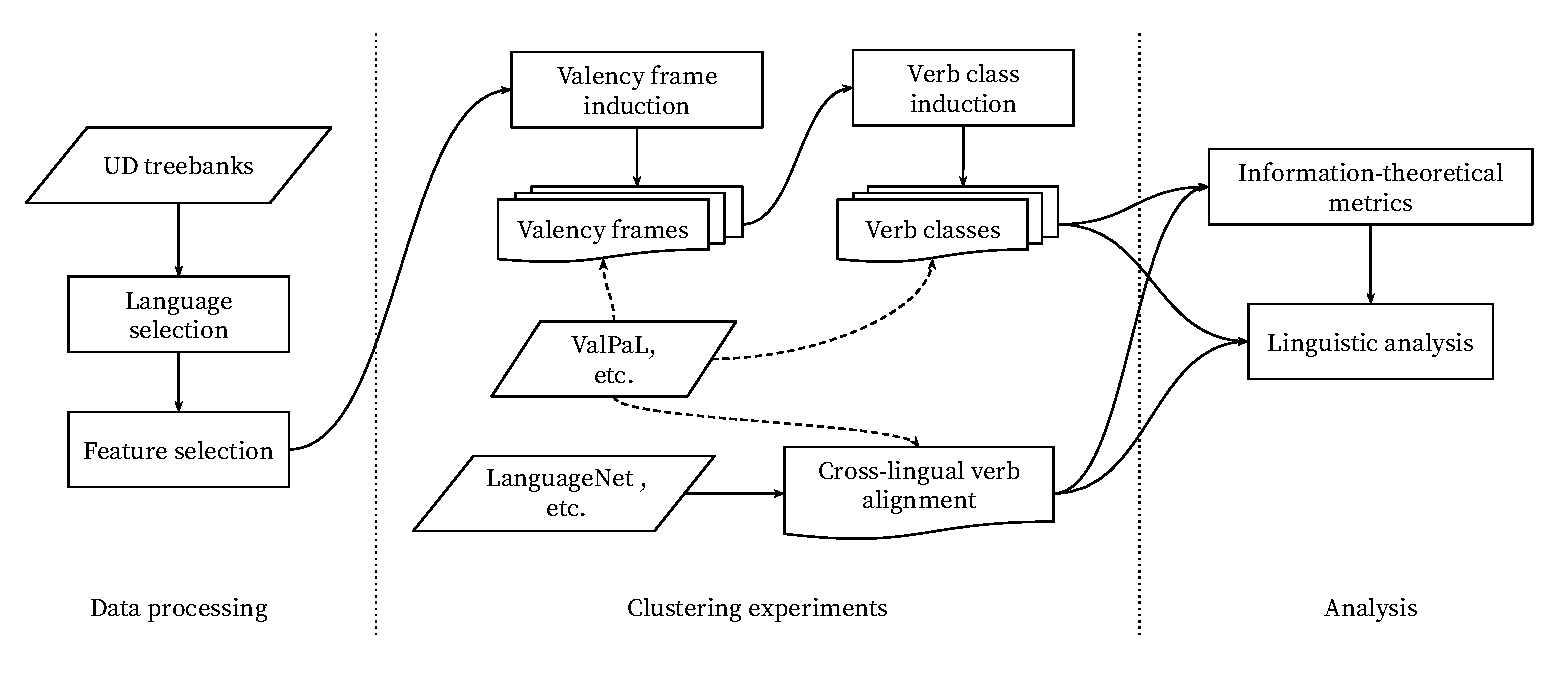
\includegraphics{figures/proposal_flowchart.pdf}
    \end{adjustbox}
    \caption{Flowchart depicting the data sources and processes as described in the proposal. Dotted lines depict validation steps.}\label{fig:flowchart}
\end{figure}

The work plan for the thesis is shown in the flowchart in Fig.~\ref{fig:flowchart}. The project with most of the specific steps already discussed in \S\ref{sec:methodology} is divided into the data processing stage, the clustering experiments stage, and the analysis stage. As far as the timeline is concerned, this thesis study is intended to be completed within roughly three months after the submission of this proposal, with a statutory maximum of six months. Given the preference for a more speedy completion, an iterative process is envisioned and priority will be put on completing a functional pipeline of the computational part already in the first month of the work, i.e. January, allowing for more flexibility later in the project. Iterative improvements will then be made upon the code and alternate methods tested. The primary experimental parts should conclude by the end of second month to allow for time needed for analysis, write-up and revisions in the final month. 
